% Created 2017-11-17 Fri 18:28
% Intended LaTeX compiler: pdflatex
\documentclass[presentation]{beamer}
\usepackage[utf8]{inputenc}
\usepackage[T1]{fontenc}
\usepackage{graphicx}
\usepackage{grffile}
\usepackage{longtable}
\usepackage{wrapfig}
\usepackage{rotating}
\usepackage[normalem]{ulem}
\usepackage{amsmath}
\usepackage{textcomp}
\usepackage{amssymb}
\usepackage{capt-of}
\usepackage{hyperref}
\usetheme{default}
\author{Shamlik}
\date{\today}
\title{MQTT using Python}
\hypersetup{
 pdfauthor={Shamlik},
 pdftitle={MQTT using Python},
 pdfkeywords={},
 pdfsubject={},
 pdfcreator={Emacs 24.5.1 (Org mode 9.0.9)}, 
 pdflang={English}}
\begin{document}

\maketitle
\begin{frame}{Outline}
\tableofcontents
\end{frame}


\begin{frame}[label={sec:orgf079412}]{One -- Intro}
\begin{block}{Lightweight pub/sub messaging}
\begin{itemize}
\item Andy Stanford(IBM),Arlen Nipper
\item Oil Pipeline telemetry systems - satellite
\item 1999 - Royalty free in 2010
\item MQTT - TCP/IP
\item MQTT-SN UDP/ZigBee (2013)
\end{itemize}
\end{block}
\end{frame}


\begin{frame}[label={sec:org4dfd9dd}]{Two -- Arch}
\begin{block}{Pub/Sub}
\begin{center}
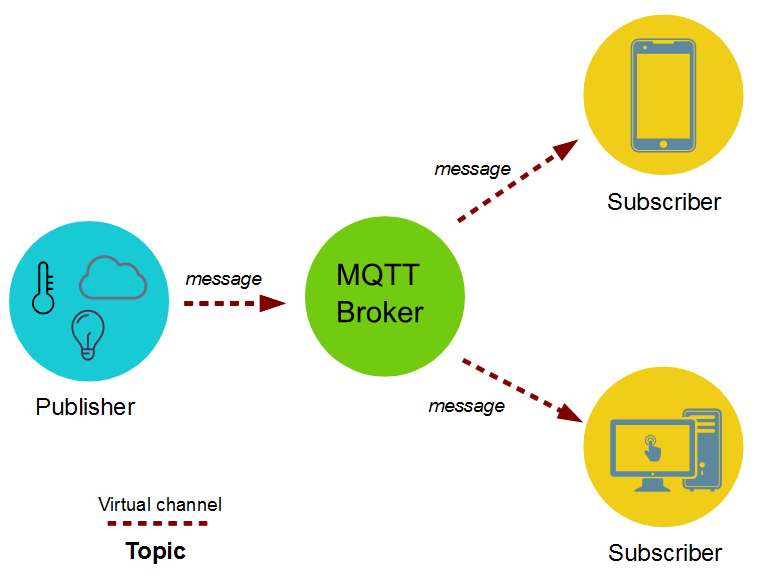
\includegraphics[width=.9\linewidth]{mqtt_arch.png}
\end{center}
\begin{itemize}
\item Three -- Comparison
\end{itemize}
\end{block}
\begin{block}{Pros}
\begin{itemize}
\item Lightweight packet structure
\item Conserve both memory usage and power
\item Reliable on Unreliable networks
\item Many-to-many broadcast
\item QOS support
\end{itemize}
\end{block}
\begin{block}{Cons}
\begin{itemize}
\item Uses TCP, Always on
\item Broker Resource utilization
\end{itemize}
\end{block}
\end{frame}
\end{document}
